\subsection{Алгоритмы оценки параметров широкополосного сигнала сигнала}

\subsubsection{Коррелятор}

\paragraph{Последовательный коррелятор}
\label{sec1_serial}
Данный алгоритм в некоторых источниках так же называется согласованным фильтром. В \cite{sklyar} рассмотрены нюансы этих двух понятий.
В данной работе мы будем использовать понятие последовательный коррелятор. Работа коррелятора описывается математической операцией
корреляции \ref{eq:serial_corr}. Сигнал коррелируется с локальной копией и на выходе коррелятора получается значение, отражающее
степень совпадения сигналов. Не трудно представить, что сигнал с хорошими корреляционными свойствами должен обладать высоким значением
корреляции когда сигналы синхронизированы и минимальным значением в любом другом случае (фаза ПСП-кода не выровнена - :отсутствие сигнала).

\begin{equation}
	\label{eq:serial_corr}
	y(n)=\sum\limits_{m=0}^{N-1}{x(m)h(n+m)}
\end{equation}
где: ${x(m)}$ - принятый сигнал, а ${h(n)}$ не импульсная характеристика системы, а локальная копия сигнала.

\paragraph{Параллельный коррелятор}
\label{sec1_fft}
Вычисление циклической свертки через дискретное преобразование Фурье (ДПФ) является достаточно популярным методом
в программных приемниках, так как позволяет существенно 
уменьшить количество элементарных операций при вычислении. Но как показано в \cite{tsui, oppenheim} можно достаточно просто
перейти от свертки к циклической корреляции. Так как этот метод является самым популярным в программных приемниках, рассмотрим его
подробнее.

Обозначим импульсный отклик системы через $h(n)$, а через ${x(n)}$ - входной сигнал. Тогда выходной сигнал в дискретном
временной домене можно записать как:
\begin{equation}
	\label{eq:fft_conv}
	y(n)=\sum\limits_{m=0}^{N-1}{x(m)h(n-m)}
\end{equation}

Стоит отметить, что в \ref{eq:fft_conv} сдвиг во времени является циклическим, поскольку дискретные операции являются циклическими.
Возьмем ДПФ от \ref{eq:fft_conv}
\begin{center}
\begin{eqnarray}
	\label{eq:fft_conv_fft}
	Y(k) & = & \sum\limits_{n=0}^{N-1}\sum\limits_{m=0}^{N-1}{x(m)h(n-m)e^{(-j2\pi{kn})/N}}=\nonumber \\
	& = & \sum\limits_{m=0}^{N-1}{x(m)}[\sum\limits_{n=0}^{N-1}h(n-m)e^{(-j2\pi{(n-m)}k)/N}]e^{(-j2\pi{m}k)/N}=\\
	& = & H(k)\sum\limits_{m=0}^{N-1}e^{(-j2\pi{m}k)/N} = X(k)H(k)\nonumber 
\end{eqnarray}
\end{center}
Из уравнения \ref{eq:fft_conv_fft} легко видеть, что это не линейная свертка. В линейной свертке для входного сигнала размером в ${N}$ точек,
результат будет из ${2N-1}$ точек. А в уравнении выше, результатом является всего ${N}$ точек.
Это проявление циклической природы ДПФ.

Алгоритм детектирования не использует свертку, он использует корреляцию, которая отличается от свертки. Корреляция
между $x(n)$ и $h(n)$ может быть записана как:
\begin{equation}
	\label{eq:fft_corr}
	z(n) = \sum\limits_{m=0}^{N-1}{x(m)h(n+m)}
\end{equation}

Единственным отличаем между \ref{eq:fft_conv} и \ref{eq:fft_corr} является знак перед $m$ в ${h(n+m)}$.
В случае детектирования сигнала, $h(n)$ является локальной копией сигнала, а не импульсной характеристикой.
Произведем ДПФ над $z(n)$:
\begin{center}
\begin{eqnarray}
	\label{eq:fft_corr_fft}
	Z(k) & = & \sum\limits_{n=0}^{N-1}\sum\limits_{m=0}^{N-1}{x(m)h(n+m)e^{(-j2\pi{kn})/N}}=\nonumber \\
	& = & \sum\limits_{m=0}^{N-1}{x(m)}[\sum\limits_{n=0}^{N-1}h(n+m)e^{(-j2\pi{(n+m)}k)/N}]e^{(j2\pi{m}k)/N}=\\
	& = & H(k)\sum\limits_{m=0}^{N-1}e^{(j2\pi{m}k)/N} = X(k)H^{-1}(k)\nonumber 
\end{eqnarray}
\end{center}
где ${X^{-1}(k)}$ - обратное ДПФ. Уравнение \ref{eq:fft_corr_fft} можно записать как:

\begin{equation}
	\label{eq:fft_corr_fft_rev}
	Y(k) = \sum\limits_{n=0}^{N-1}\sum\limits_{m=0}^{N-1}{x(n+m)h(m)e^{(-j2\pi{kn})/N}}=X^{-1}(k)H(k)
\end{equation}

Если сигнал $x(n)$ реальный, то $x(n) = x^*(n)$, где ${*}$ - операция комплексного сопряжения. Используя данное соотношение,
значение $Z(k)$ может быть записано:
\begin{equation}
	\label{eq:fft_magnitude}
	|Z(k)|=|H^*(k)X(k)|=|H(k)X(k)^*|
\end{equation}
Данное соотношение может быть использовано для нахождения значения циклической корреляции между входным сигналом и 
локальной копией.

\paragraph{ФАПЧ}
Программные приемники системы Navstar GPS рассмотрены в \cite{tsui, akos-book}.
После стадии детектирования сигнала, оценка частоты для заданного источника поступает в модуль уточнения частоты.
Уточненная частота и фаза ПСП поступают в ФАПЧ.

Одним из параметров системы ФАПЧ является шумовая полоса.
Этот параметр определяет количество теплового шума попадающего в систему ФАПЧ. Широкая шумовая полоса позволяет системе ФАПЧ быстро войти в синхронизм,
но также ведет к существенному ухудшению характеристик системы ФАПЧ за счет возрастания уровня теплового шума.

Область допустимой расстройки частоты, в пределах которой обеспечивается захват, при коэффициенте демпфирования ${\zeta>0.3}$ определяется как
\cite{spilker-book}:
\begin{center}
\begin{equation}
	\label{eq:corr_pll_band}
	\Delta \omega_m = 2 \omega_n (\zeta + 0.6)
\end{equation}
\end{center}
где ${\omega_m}$ - собственная частота системы ФАПЧ, ${\zeta}$ - коэффициент демпфирования,

В \cite{tsui, spilker-book} предложено брать ${\zeta=0.707}$, тогда ${\Delta \omega_m = 2.614 \omega_n}$.
Собственная частота модуля фазовой автоподстройки частоты вычисляется по формуле:
\begin{center}
\begin{equation}
	\label{eq:corr_pll_freq}
	\omega_n = \frac{8 \zeta B_L}{4 \zeta^2 + 1} 
\end{equation}
\end{center}
где ${B_L}$ - шумовая полоса.

Традиционный подход детектирования сигнала предусматривает корреляцию входного сигнала и набора локальных копий сигнала с шагом 1 кГц.
Для стационарного приемника Navstar GPS диапазон смещения частоты, обусловленный допплеровским эффектом, может находится в диапазоне
${\pm 5}$ кГц \cite{tsui}.  Таким образом при шаге 1 кГц необходимо провести поиск в 11 ячейках. В каждой ячейке нам необходимо ${N}$-комплексных умножений.
Для наземных приемников типовое значение  ${B_L=20}$ Гц \cite{tsui, akos-book}. Область синхронизации из выражения \ref{eq:corr_pll_band} и 
\ref{eq:corr_pll_freq}.
${\Delta \omega_m \approx 100}$ Гц. Таким образом необходима стадия уточнения частоты.

Схема традиционного приемника изображена на рисунке \ref{pic:corr_scheme}.
\begin{figure}[H]
	\center\scalebox{1}{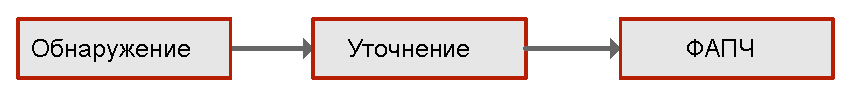
\includegraphics[width=1\linewidth]{corr_scheme.eps}}
	\caption{Схема традиционного приемника}
	\label{pic:corr_scheme}
\end{figure}

Количество комплексных умножений, требуемых для оценки частоты одного источника параллельным коррелятором: ${OP_{FFT} = 12NlogN + 11N}$

Алгоритм уточнения частоты описан в \cite{tsui}. Следует отметить, что данный алгоритм основан на усреднении фазы и требует дополнительной
оперативной памяти (ОЗУ) приемника для хранения 5 миллисекунд данных при обработке одного источника. Оперативная память потребляет значительное количество энергии,
поэтому снижение количества необходимой ОЗУ является важной задачей при разработке портативных приемников.
Так же обработка 5 мс данных повышает встретить переход бита внутри данных – это ведет к дополнительным сложностям при реализации программных
приемников сигнала Navstar GPS.

Алгоритм уточнения частоты описан в \cite{tsui}. Следует отметить, что данный алгоритм основан на усреднении фазы и требует дополнительной
оперативной памяти (ОЗУ) приемника для хранения 5 миллисекунд данных при обработке одного источника. Оперативная память потребляет значительное количество
энергии, поэтому снижение количества необходимой ОЗУ является важной задачей при разработке портативных приемников. Также обработка 5 мс данных повышает
вероятность встретить переход бита внутри данных – это ведет к дополнительным сложностям при реализации программных приемников сигнала Navstar GPS.

Количество умножений, требуемых для уточнения частоты одного источника:
\begin{itemize}
	\item Повторная модуляция 5 мс данных: ${5N}$ умножений;
	\item Повышение точности до 400Гц: ${6N}$ умножений;
	\item Вычисление ДПФ в частотной позиции на длине: ${10N}$ умножений.
\end{itemize}

Количество умножений, требуемых для уточнения частоты одного источника: ${OP_{FINE} = 21N}$

\newpage
